\documentclass{article}
\usepackage[utf8]{inputenc}
\usepackage{graphicx}
\usepackage{parskip}
\usepackage{xcolor}
\usepackage{textcomp}
\usepackage{hyperref}
\hypersetup{
    colorlinks=true,
    linkcolor=blue,
    filecolor=magenta,      
    urlcolor=cyan,
}
\usepackage{listings}
\lstset{language=C,
                backgroundcolor = \color{lightgray},
                showstringspaces = false,
                basicstyle=\ttfamily,
                keywordstyle=\color{blue}\ttfamily,
                stringstyle=\color{red}\ttfamily,
                commentstyle=\color{green}\ttfamily,
                morecomment=[l][\color{magenta}]{\#}
}

\title{The Timed Bomb - Code Documentation}
\author{By \\ Umang Deshpande and Akshay Hegde}
\date{June 2017}

\begin{document}
\maketitle

\subsection{Program Code}
\qquad The git repository for the complete code can be found \href{https://github.com/eYSIP-2017/eYSIP-2017_Game_Development-TI-RTOS/tree/master/Documentation/Timer\%20Bomb/Timer\%20Bomb\%20-\%20Code/TimedBomb_Final}{here}. It contains the complete project folder used in CCS. 
\begin{itemize}
  \item The console support libraries are present in the \href{https://github.com/eYSIP-2017/eYSIP-2017_Game_Development-TI-RTOS/tree/master/Documentation/Timer\%20Bomb/Timer\%20Bomb\%20-\%20Code/TimedBomb_Final/Console}{Console} folder. 
  \item timedbomb.c is the main file. This contains the Statechart and  the Timer Bomb abstraction.
\end{itemize}

\section{Main Code}
\qquad Firstly, following headers are included:
  \begin{lstlisting}[basicstyle = \small, language = C]
#include <stdint.h>
#include <stdbool.h>
#include "inc/hw_memmap.h"
#include "inc/hw_types.h"
#include "driverlib/interrupt.h"
#include "inc/tm4c123gh6pm.h"
#include "driverlib/sysctl.h"
#include "driverlib/gpio.h"
#include "driverlib/pin_map.h"
#include "driverlib/timer.h"
/*
* Console includes all graphics images and glcd functions
used to display graphics
*/
#include "Console/setupConsole.h"
#include "Console/glcdFunctions.h"
#include "Console/glcdLibrary.h"
  \end{lstlisting}
\begin{itemize}
  \item \texttt{stdint.h} Headers allow use of \texttt{uint32} variables, stdbool allows use of \texttt{stdbool.h} variables.
  \item For the timer and timer interrupt functions used in Timer ISR(Task Scheduler), \texttt{timer.h} and \texttt{hw\_memmap.h} are used.Pin mapping, gpio related functions and board specific functions are used from \texttt{driverlib/pin\_map.h},\\  \texttt{driverlib/gpio.h} and \texttt{tm4c123gh6pm.h} respectively.
  \item The Console headers provide developer level functions to the console, so that initialization can be performed using a single function \texttt{\_init\_()}. And GLCD functions for direct display of fonts and graphic are obtained from \texttt{glcdFuctions.h} header.

  \item \texttt{glcdLibrary.h} Contains various different images in the form of hex arrays to be displayed on screen.
\end{itemize}
\newpage
\qquad Following this, define all global variables are defined as follows:
  \begin{lstlisting}[basicstyle = \small, language = C]
/*
 * Global Variables
 */
uint8_t volatile mode;

/*
 * sw1_status=DOWN,sw2_status=UP,sw3_status=LEFT,
   sw4_status=RIGHT
 * password bits
 * passbit1=down,passbit2=up,passbit3=left
 */

uint32_t volatile sw1_status,sw2_status,sw3_status,sw4_status;
uint8_t volatile flag1=0,flag3=0,flag4=0,flag5=0,flag6=0,
passbit1=0,passbit2=0,passbit3=0;
/*
 * Timer Digit Display positions
 */
int bit_pos0=0,bit_pos1=2,bit_pos2=0,bit_pos3=0;
/*
 * Time Counter
 */
int cal_time=120;
  \end{lstlisting}
\begin{itemize}
  \item \texttt{mode},is used for switching into different modes. \texttt{sw1\_status, sw2\_status, sw3\_status,sw4\_status} are the variables which holds the status of switches connected to ports in sequence as  DOWN,UP,LEFT and RIGHT respectively. 
  \item \texttt{flag1} is flag which ensures the display of frame1 in idle mode.
  \item \texttt{flag3} when set mode changes from idle to setTimer.
  \item \texttt{flag4} when set mode changes from setTimer to autoTimer.
  \item \texttt{flag5} when set mode changes to bombExplode.
  \item \texttt{flag6} when set mode changes to idle.
  \item \texttt{passbit1},\texttt{passbit2} and \texttt{passbit3} checks for correct password to diffuse the bomb.
  \item \texttt{bit\_pos0}, \texttt{bit\_pos1}, \texttt{bit\_pos2} and \texttt{bit\_pos3}holds the 4 digit timer bits.
\end{itemize}
\qquad All the different states for the various state machines used are enlisted as follows:
  \begin{lstlisting}[basicstyle = \small, language = C]
/*
 * Enumeration of States for Each Switch(for debouncing)
 */
enum states{S_idle0,S_press0,S_release0};
enum events{E_npress0,E_press0};
enum states1{S_idle1,S_press1,S_release1};
enum events1{E_npress1,E_press1};
enum states2{S_idle2,S_press2,S_release2};
enum events2{E_npress2,E_press2};
enum states3{S_idle3,S_press3,S_release3};
enum events3{E_npress3,E_press3};
/*
 * Enumeration of states for the Bomb(for State Machine)
 */
enum modes{idle,setTimer,autoTimer,bombExplode,bombDiffused};
// State Initialization
uint8_t volatile currentstate0=S_idle0;
uint8_t volatile currentstate1=S_idle1;
uint8_t volatile currentstate2=S_idle2;
uint8_t volatile currentstate3=S_idle3;
  \end{lstlisting}
\begin{itemize}
  \item \texttt{enum states and events}. This is enumeration of states for each switch for debouncing. \texttt{States} represent the different states in which the switch can be, and \texttt{events} represent the two events \texttt{switch pressed} or \texttt{switch not pressed}.
  \item \texttt{modes} represents the different modes the bomb Timer can be. These are the different states.
  \item initially all the switches are in idle state.
      \begin{lstlisting}[basicstyle = \small, language = C]
/*
 * Function prototyping
 */
int KeyPress0(void);
int KeyPress1(void);
int KeyPress2(void);
int KeyPress3(void);
void statemachine0(int);
void statemachine1(int);
void statemachine2(int);
void statemachine3(int);
void exitaction0(int);
void exitaction1(int);
void exitaction2(int);
void exitaction3(int);
void enteraction0(int);
void enteraction1(int);
void enteraction2(int);
void enteraction3(int);
void selectmode(void);
  \end{lstlisting}
  \item Function prototyping is done to avoid warnings.
      \begin{lstlisting}[basicstyle = \small, language = C]
void bombDiffusedScreen(void)
{
    int i,j,k=0;
    // Disable Timer
    TimerDisable(TIMER0_BASE, TIMER_A);
    TimerDisable(TIMER1_BASE, TIMER_A);
    IntMasterDisable();

    glcd_cleardisplay();
    // Display Smiley
    for(i=2;i<6;i++)
    {
        for(j=48;j<80;j++)
        {
            glcd_set_page_col(i,j);
            glcd_data(smiley[k]);
            k++;
        }
    }
    SysCtlDelay(10000000);
    glcd_cleardisplay();
    // Restart Timer
    IntMasterEnable();
    TimerEnable (TIMER0_BASE, TIMER_A);
    TimerEnable (TIMER1_BASE, TIMER_A);

}
  \end{lstlisting}
  \item \texttt{bombDiffusedScreen()}. This function represents the actions to be performed in bombDiffused state. First the the interrupt is disabled to avoid jumping of control. Glcd is cleared and then smiley is displayed.
      \begin{lstlisting}[basicstyle = \small, language = C]
void bombExplosionScreen(void)
{
    int i,j,k=0,l=0;
    // Stop Timer
    IntMasterDisable();
    TimerDisable(TIMER0_BASE, TIMER_A);
    TimerDisable(TIMER1_BASE, TIMER_A);
    while(k<4)
    {
      // Display Explosion Animation(4 screen animation)
        for(i=0;i<8;i++)
        {
            for(j=0;j<128;j++)
            {
                glcd_set_page_col(i,j);
                glcd_data(explosion[k][l]);
                l++;
            }
        }
        l=0;
        glcd_cleardisplay();
        k++;
    }
    glcd_cleardisplay();
    k=0;
    for(i=2;i<6;i++)
    {
      // Display Skull(on Death)
        for(j=48;j<80;j++)
        {
            glcd_set_page_col(i,j);
            glcd_data(skull[k]);
            k++;
        }
    }
    SysCtlDelay(10000000);
    glcd_cleardisplay();
    // Restart Timer
    IntMasterEnable();
    TimerEnable (TIMER0_BASE, TIMER_A);
    TimerEnable (TIMER1_BASE, TIMER_A);

}
  \end{lstlisting}
  \item \texttt{ bombExplosionScreen()}. This function displays bomb explosion animation and skull animation.
      \begin{lstlisting}[basicstyle = \small, language = C]
void eval_time()
{
    bit_pos0=0;
    bit_pos1=cal_time/60;
    bit_pos3=(cal_time%60)%10;
    bit_pos2=(cal_time%60)/10;

}
  \end{lstlisting}
  \item \texttt{eval\_time()}. This function calculates the timer value in 4 bits, with bitpos0 being msb. 
      \begin{lstlisting}[basicstyle = \small, language = C]
void Timer0IntHandler(void)
{
// Clear the timer interrupt
TimerIntClear(TIMER0_BASE, TIMER_TIMA_TIMEOUT);

switch(mode){
  case setTimer:
      glcd_frame2_write();
      glcd_frame3_write();
      break;
  case autoTimer:
   // In autoTimer Mode, evaluate time and display
   the timer bits
      glcd_digit_write(bit_pos0,0);
      glcd_digit_write(bit_pos1,1);
      glcd_digit_write(bit_pos2,2);
      glcd_digit_write(bit_pos3,3);
      clear_section_glcd(2,0,78);
      glcd_bomb_write();
  // Switch to Bomb Explosion on Timeout
      if(cal_time==0)
      {
        flag5=1;
        flag4=0;
      }
  // Decrement Time
      if(cal_time>0)
      {
        cal_time--;
      }
      eval_time();
      break;
}
}
  \end{lstlisting}
  \item \texttt{Timer0IntHandler}.It is the Isr function called when timer0 overflows. Itis used to create a clock ticking at 1 second. Depending upon the mode the action is performed. In setTimer mode the instruction are displyed. In autoTimer mode the 4 bit Timer is Displayed.
  \item If the Timer value reaches zero the mode changes to bombExplode and flag5 is Set.
  \item The timer count decreases by 1 second.
      \begin{lstlisting}[basicstyle = \small, language = C]
void updateGLCD(void)
{
   //select the mode
    selectmode();
    switch(mode){
      case idle:
          if(flag1 == 0)
          {
            // Display first time once
              cal_time=120;
              glcd_frame1_write();
              flag1=1;
          }
          break;
      case setTimer:
      // In setTimer mode display the timer
      // Display set time with continuous refresh
      glcd_digit_write(bit_pos0,0);
      glcd_digit_write(bit_pos1,1);
      glcd_digit_write(bit_pos2,2);
      glcd_digit_write(bit_pos3,3);
    }
}
  \end{lstlisting}
  \item \texttt{updateGLCD}. This function updates the Glcd depending upon the mode the bomb Timer is in. If the timer is in mode 1 frame1 is displayed, if in setTimer mode 4 bit Timer is Displayed.
      \begin{lstlisting}[basicstyle = \small, language = C]
void Timer1IntHandler(void)
{
  // Clear raised Timer 1 Interrupt
    TimerIntClear(TIMER1_BASE, TIMER_TIMA_TIMEOUT);

    statemachine0(KeyPress0());
    statemachine1(KeyPress1());
    statemachine2(KeyPress2());
    statemachine3(KeyPress3());

     updateGLCD();
     switch(mode){
       case(bombExplode):
       // Timer Timeout
          bombExplosionScreen();
          passbit1=0;
          passbit2=0;
          passbit3=0;
          flag5=0;
          flag6=1;
          flag1=0;
          break;
       case(bombDiffused):
       //Passcode Entered
          bombDiffusedScreen();
          passbit1=0;
          passbit2=0;
          passbit3=0;
          flag6=1;
          flag5=0;
          flag1=0;
          flag4=0;
          break;
     }
}
  \end{lstlisting}
  \item \texttt{Timer1IntHandler}.It is the Timer1 Isr used for switch debouncing and updation of glcd.
      \begin{lstlisting}[basicstyle = \small, language = C]
int KeyPress0(void)
{
    sw1_status = GPIOPinRead(GPIO_PORTF_BASE,GPIO_PIN_4);
    if ((sw1_status)!=(GPIO_PIN_4)) // switch
    pressed down key
    {
         return E_press0;
    }
    else if((sw1_status)==(GPIO_PIN_4))
    {
        return E_npress0;
    }

}

void statemachine0(int event)
{
    int nextstate0=currentstate0;
    switch(currentstate0)
    {
    case S_idle0:
        switch(event)
        {
        case E_press0:
            nextstate0=S_press0;
            break;
        case E_npress0:
            nextstate0=S_idle0;
            break;
        }
        break;
    case S_press0:
        switch(event)
        {
        case E_press0:
             nextstate0=S_release0;
             break;
        case E_npress0:
             nextstate0=S_idle0;
             break;
        }
        break;
    case S_release0:
        switch(event)
        {
        case E_press0:
            nextstate0=S_release0;
            break;
        case E_npress0:
            nextstate0=S_idle0;
        }
        break;
        default:
            break;
    }
    if((currentstate0)!=(nextstate0))
    {
        if(!((currentstate0==S_press0)&&(nextstate0==S_idle0)))
        {
        exitaction0(currentstate0);
        currentstate0=nextstate0;
        }
    }
}
  \end{lstlisting}
  \item \texttt{Keypress}. This function checks for the keypress for a switch.Keypress0, Keypress1, Keypress2, Keypress3 corresponds to DOWN,UP,LEFT and RIGHT switches. It return the value depending upon the switch press.
  \item \texttt{statemachine}. This function implements the switch debouncing statemachine. It corresponds to each switch same as with Keypress.
  \item For each switch keypress and statemachine functions are
  written. 
      \begin{lstlisting}[basicstyle = \small, language = C]
void exitaction0(int state)
{
    if(state == S_release0)
    {
      if(mode==setTimer)
      {
          if(cal_time<=10)
          {
              cal_time=120;

          }
          else
          {
          cal_time--;
          }
          eval_time();
          updateGLCD();

      }
      if((mode==autoTimer)&&(passbit2==1))
      {
          passbit1=0;
          passbit2=0;
          passbit3=0;
      }
      if(mode==autoTimer)
      {
          passbit1=1;
      }
    }
}
  \end{lstlisting}
  \item \textttt{exitaction0}.This function represents the action to be performed when DOWN switch is pressed. In mode setTimer the DOWN key press decrements the 4 bit Timer. In autoTimer mode sets the passbit1 to 1 if pressed first else clears the password.
      \begin{lstlisting}[basicstyle = \small, language = C]
void exitaction1(int state)
{
    if(state == S_release1)
    {
      if(mode==setTimer)
      {
          if(cal_time>=120)
          {
              cal_time=10;

          }
          else
          {
          cal_time++;
          }
          eval_time();
          updateGLCD();

      }
      if((mode==autoTimer)&&(passbit1==1))
      {
          passbit2=1;
      }
    }
}
  \end{lstlisting}
  \item \textttt{exitaction1}.This function represents the action to be performed when UP switch is pressed. In mode setTimer the DOWN key press increments the 4 bit Timer. In autoTimer mode sets the passbit2 to 1 if pressed second. 
      \begin{lstlisting}[basicstyle = \small, language = C]
void exitaction2(int state)
{
    if(state == S_release2)
    {
      if(mode == idle)
      {
          flag3=1;
          glcd_cleardisplay();
          eval_time();
          glcd_digit_write(bit_pos0,0);
          glcd_digit_write(bit_pos1,1);
          glcd_digit_write(bit_pos2,2);
          glcd_digit_write(bit_pos3,3);

      }
      if((mode == autoTimer)&&(passbit2 == 1))
      {
          passbit3=1;
      }
      else if((mode == autoTimer)&&(passbit1 == 1))
      {
          passbit1=0;
          passbit2=0;
          passbit3=0;
      }
    }
}
  \end{lstlisting}
  \item \textttt{exitaction1}.This function represents the action to be performed when LEFT switch is pressed. In mode idle the LEFT key press changes the mode to setTimer and displays the Timer. In autoTimer mode sets the passbit2 to 1 if pressed third else clears it.  
      \begin{lstlisting}[basicstyle = \small, language = C]
void exitaction3(int state)
{
    if(state == S_release3)
    {
      if(mode==setTimer)
      {
      flag4=1;
      flag3=0;
      }
      if((mode==autoTimer))
      {
          passbit1=0;
          passbit2=0;
          passbit3=0;
      }
    }
}
  \end{lstlisting}
  \item \textttt{exitaction2}.This function represents the action to be performed when RIGHT switch is pressed. In mode setTimer the RIGHT key press changes the mode to autoTimer. In autoTimer if pressed clears password.
    \begin{center}
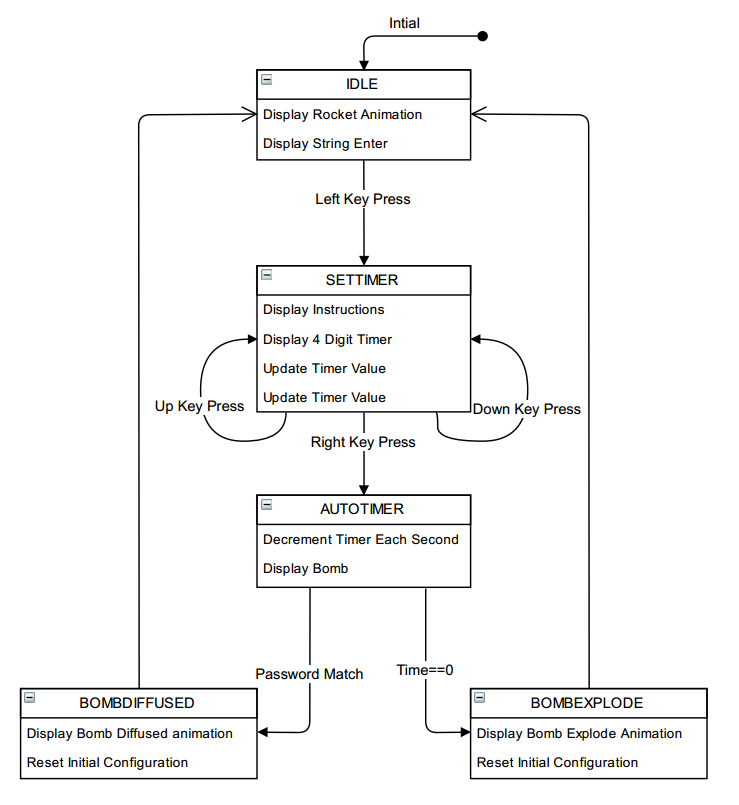
\includegraphics[width=10cm,height=10cm]{BombTimerStateChart}
\\{\small Fig a: TimerState Statechart} 
\end{center}
      \begin{lstlisting}[basicstyle = \small, language = C]
void selectmode(void)
{
/*
 * if password bit3 is 1 then mode is bombDiffused
 */
    if(passbit3==1)
    {
        mode=bombDiffused;
    }
    /*
     * If flag3 is set then mode is setTimer
     */
    else if(flag3==1)
   {
       mode=setTimer;
   }
    /*
     * If flag4=1 is set then mode is autoTimer
     */
   else if(flag4==1)
   {
       mode=autoTimer;
   }
    /*
     * If flag5 is set then mode is bombExplode
     */
   else if(flag5==1)
   {
       mode=bombExplode;
   }
    /*
     * if flag6 is set then mode is idle
     */
   else if(flag6==1)
   {
       mode=idle;
}
  \end{lstlisting}
  \item \textttt{selectmode}.This function selects the mode depending upon the status of flags.
      \begin{lstlisting}[basicstyle = \small, language = C]
void main()
{

    setup();
    glcd_init();
    glcd_cleardisplay();
    /*
     * enable the timer 0 and 1
     */
    IntEnable(INT_TIMER0A);
    TimerIntEnable(TIMER0_BASE, TIMER_TIMA_TIMEOUT);
    IntEnable(INT_TIMER1A);
    TimerIntEnable(TIMER1_BASE, TIMER_TIMA_TIMEOUT);
    IntMasterEnable();

    TimerEnable (TIMER0_BASE, TIMER_A);
    TimerEnable (TIMER1_BASE, TIMER_A);
    /*
     * initial mode is idle
     */
    mode=idle;

    while(1)
    {
       /*
        * select mode continuously
        */
        selectmode();

    }

}
  \end{lstlisting}
  \item \textttt{main}.This function calls the setup files and glcd initialization.
   \item It enables the Timer0 and Timer1.
   \item Sets initial mode as Idle and continuously selects mode.
  \end{itemize}
This is the complete code for the Timed Bomb Controller, with a state machine implementation.
\end{document}
